\section{Theoretical Result}\label{sec:fc}
Our goal is to characterise `what is learnt in the gates of a DNN with ReLUs'. To this end, we use the DGN setup where the gates and weights are separate. Specifically, the DNN with ReLUs whose gates we want to examine is the feature network in the DGN. We then measure the information in the gates by keeping the gates fixed and training the value network and measuring the test performance of the value network. It was shown in [\citenum{npk}] that if the gates are fixed  (i.e., with reference to \Cref{prop:ntks}, $\kf=0$), for fully connected DGN, the NTK simplifies as $\text{NTK}(x,x')\propto \text{NPK}(x,x') = \ip{x,x'}\cdot {\bf{overlap}}(x,x')$. In this section, we state three results, where in \Cref{th:main} we `re-write' Theorem~$5.1$ in [\citenum{npk}] to explicitise the role of gates, width and depth, to yield a simple product of kernels expression (unnoticed in prior works).  \Cref{th:mainconv} covers the case of convolutions with pooling and \Cref{th:mainres} covers the case residual networks with skip connections.

\textbf{Note 1.} The gates of the DGN can also be tuned, in which case $\kf\neq \mathbf{0}$, and we reserve the study of $\kf$ for future. The results are for infinite width networks and at randomised initialisation. We use these insights as an indicator of what we can expect when we experiment with finite width networks. 

We begin with an assumption that states that the value network weights have to be statistically independent of the feature network weights at initialisation. %With reference to \Cref{prop:ntks}, since the gates fixed, it follows that $\kf=\mathbf{0}$ and we will characterise only $\kv$ which corresponds to the value network. Here, the DGN is used to study the gates of a \emph{untrained/(partially or fully) trained} DNN with ReLUs. We wish to point that the gates of the DGN can also be tuned in which case $\kf\neq \mathbf{0}$, and we reserve the study of $\kf$ for future. We now state an assumption on the value network 

%In this section, we state three results (\Cref{th:main,th:mainconv,th:mainres}) that characterise `what is learnt in the gates of a DNN with ReLUs'.  To this end, we use the DGN setup where the gates and weights are separate. Specifically, the DNN with ReLUs whose gates we want to examine becomes the feature network in the DGN. If we keep the feature network weights fixed, the gates are automatically fixed. We then characterise the information in the gates by training the value network and measuring the test performance of the value network. With reference to \Cref{prop:ntks}, since the gates fixed, it follows that $\kf=\mathbf{0}$ and we will characterise only $\kv$ which corresponds to the value network. Here, the DGN is used to study the gates of a \emph{untrained/(partially or fully) trained} DNN with ReLUs. 

\begin{assumption}\label{assmp:main}
$\Tv_0\stackrel{\text{i.i.d}}\sim\text{Bernoulli}(\frac12)$ over $\{-{\sigma},+{\sigma}\}$ and statistically independent of $\Tf_0$.
\end{assumption}
We point out that this statistical decoupling of weights and gates in \Cref{assmp:main} is unrealisable in a DNN with ReLU, however, this assumption can be trivially realised in a DGN.
\begin{theorem}[Product of Kernels Theorem]\label{th:main} Under \Cref{assmp:main}  ($\sigma=\frac{\cscale}{\sqrt{w}}$) for FC-DGN : 
\begin{align*}
\kv_{\Tdgn_0}(x,x') \ra d\cdot \cscale^{d-1} \cdot \left(\ip{ x,x'} \cdot \Pi_{l=1}^{d-1} \frac{\ip{G_l(x),G_l(x')}}w\right), \quad\text{as}\,\, w\ra\infty 
\end{align*}
\end{theorem} 
\textbf{Key Insight.} Here $\frac{\ip{G_l(x),G_l(x')}}w$ are the \emph{base kernels} measuring the \emph{\textbf{correlation of the gates}}. We show experimentally that the correlation of gates is essentially  `what is learnt in a DNN with ReLUs'.
%and $\Pi_{l=1}^{d-1} \frac{\ip{G_l(x),G_l(x')}}w$ is a product of these base kernels and hence the name `Product of Kernels Theorem'.  The base kernels are essentially measuring which we show via  We now list the roles of the two networks, weights, depth and width.

\textbf{Feature Network.} The role of this network is to process the input layer-by-layer and produce the $w$-dimensional gating features $G_l(\cdot)$. Each layer comprises of `$w$' ReLUs, and a given ReLU (i.e., gate) is `on' if the input to that layer lies on the positive half-space of hyperplane of given by the incoming weights of that ReLU. Thus the gates of a given layer are based on the angle between the input to that layer and the various hyperplanes given by the weights of that layer. Prior experiments in [\citenum{npk}] and the experiments in this paper show that the feature network, i.e., the gates hold most information, which in turn means that weights of the feature network are key.

\textbf{Value Network}. The value network implements the product of kernels by laying out the gates as masks depth-wise, and connecting them in the structure of a DNN. Note that depth-wise layout plays an important role here: for instance, if we were to concatenate the gating features as $\varphi(x)=(G_l(x),l=1,\ldots,d-1)\in\{0,1\}^{(d-1)w}$, it would have only resulted in the kernel $\ip{\varphi(x),\varphi(x')}=\sum_{l=1}^{d-1}{\ip{G_l(x),G_l(x')}}$, i.e., a \emph{sum  (not product)} of kernels. Prior experiments in [\citenum{npk}] and the experiments in this paper show that the value network can be reset and re-trained without loss of performance, which in turn means that weights of the value network are not that important.

\textbf{Note.} The above insights from \Cref{th:main} carry over to the case of DNN with ReLUs by thinking that the roles of value and feature network are performed by a single network.

\textbf{Convolutions with pooling.} Let the circular rotation of vector $x\in\R^{\din}$ by `$r$' co-ordinates be defined as $rot(x,r)(i)=x(i+ r)$, if $i+r \leq \din$ and $rot(x,r)(i)=x(i+ r-\din)$ if $i+r > \din$. Using circular convolutions with pooling results in a rotationally invariant kernel \Cref{th:mainconv}. The architecture and the notations for the network with convolutions is presented in the Appendix.
\begin{comment}
 We extend the dual view to neural network with $\dc$ convolutional layers ($l=1,\ldots,\dc$), followed by a \emph{global-average/max-pooling} layer ($l=\dc+1$) and $\dfc$ ($l=\dc+2,\ldots,\dc+\dfc+1$) fully connected  layers (see Appendix for notation). The convolutional window size is $\wconv<\din$, the number of filters per convolutional layer as well as the width of the fully connected layers is $w$. The main steps are (i) treating pooling layers like gates/masks, (ii) bundling together the paths that share the same path value (due to weight sharing in convolutions) and (iii) re-defining the NPF and NPV for these bundles. The important consequence of weight sharing (due to convolutions and pooling) is that the NPK becomes rotationally invariant resulting in \Cref{th:mainconv}.
\end{comment}
\begin{theorem}[Rotationally Invariant Kernel Theorem]\label{th:mainconv} Under \Cref{assmp:main}, for  a suitable $\bcnn$:
\begin{align*}
&\kv_{\Tdgn_0}&\ra&\quad \frac{\bcnn}{{\din}^2} \cdot \sum_{r=0}^{\din-1} \ip{x,rot(x',r)}_{\Lambda(\cdot, x,rot(x',r))},\,\, \text{as}\,\,  w\ra\infty\,\text{(for global-average-pooling)}, \\
&\kv_{\Tdgn_0}&\ra& \quad{\bcnn} \cdot \sum_{r=0}^{\din-1} \ip{x,rot(x',r)}_{\Lambda(\cdot, x,rot(x',r))},\,\, \text{as}\,\,  w\ra\infty\,\text{(for global-max-pooling)}
\end{align*}
\end{theorem}
\textbf{Remark.} $\sum_{r=0}^{\din-1} \ip{x,rot(x',r)}_{\Lambda(\cdot, x,rot(x',r))}=\sum_{r=0}^{\din-1} \left(\sum_{i=1}^{\din} x(i) rot(x',r)(i)\Lambda(i,x,x')\right)$, where the inner `$\Sigma$' is the inner product between $x$ and $rot(x',r)$ weighted by $\Lambda$ and the outer `$\Sigma$' covers all possible rotations, which results in the rotational invariance property.

\textbf{Residual Networks with Skip connections.} We consider a ResNet with `$(b+2)$' blocks and `$b$' skip connections between the blocks (left of \Cref{fig:resnet}). Each block is a fully connected (FC) DNN of depth `$\dblock$' and width `$w$'. There are combinatorially many sub-FC-DNNs within this ResNet (see \Cref{def:subfcdnn} and right of \Cref{fig:resnet}).
\FloatBarrier
\begin{figure}[h]
\begin{minipage}{0.5\columnwidth}
\resizebox{\columnwidth}{!}{
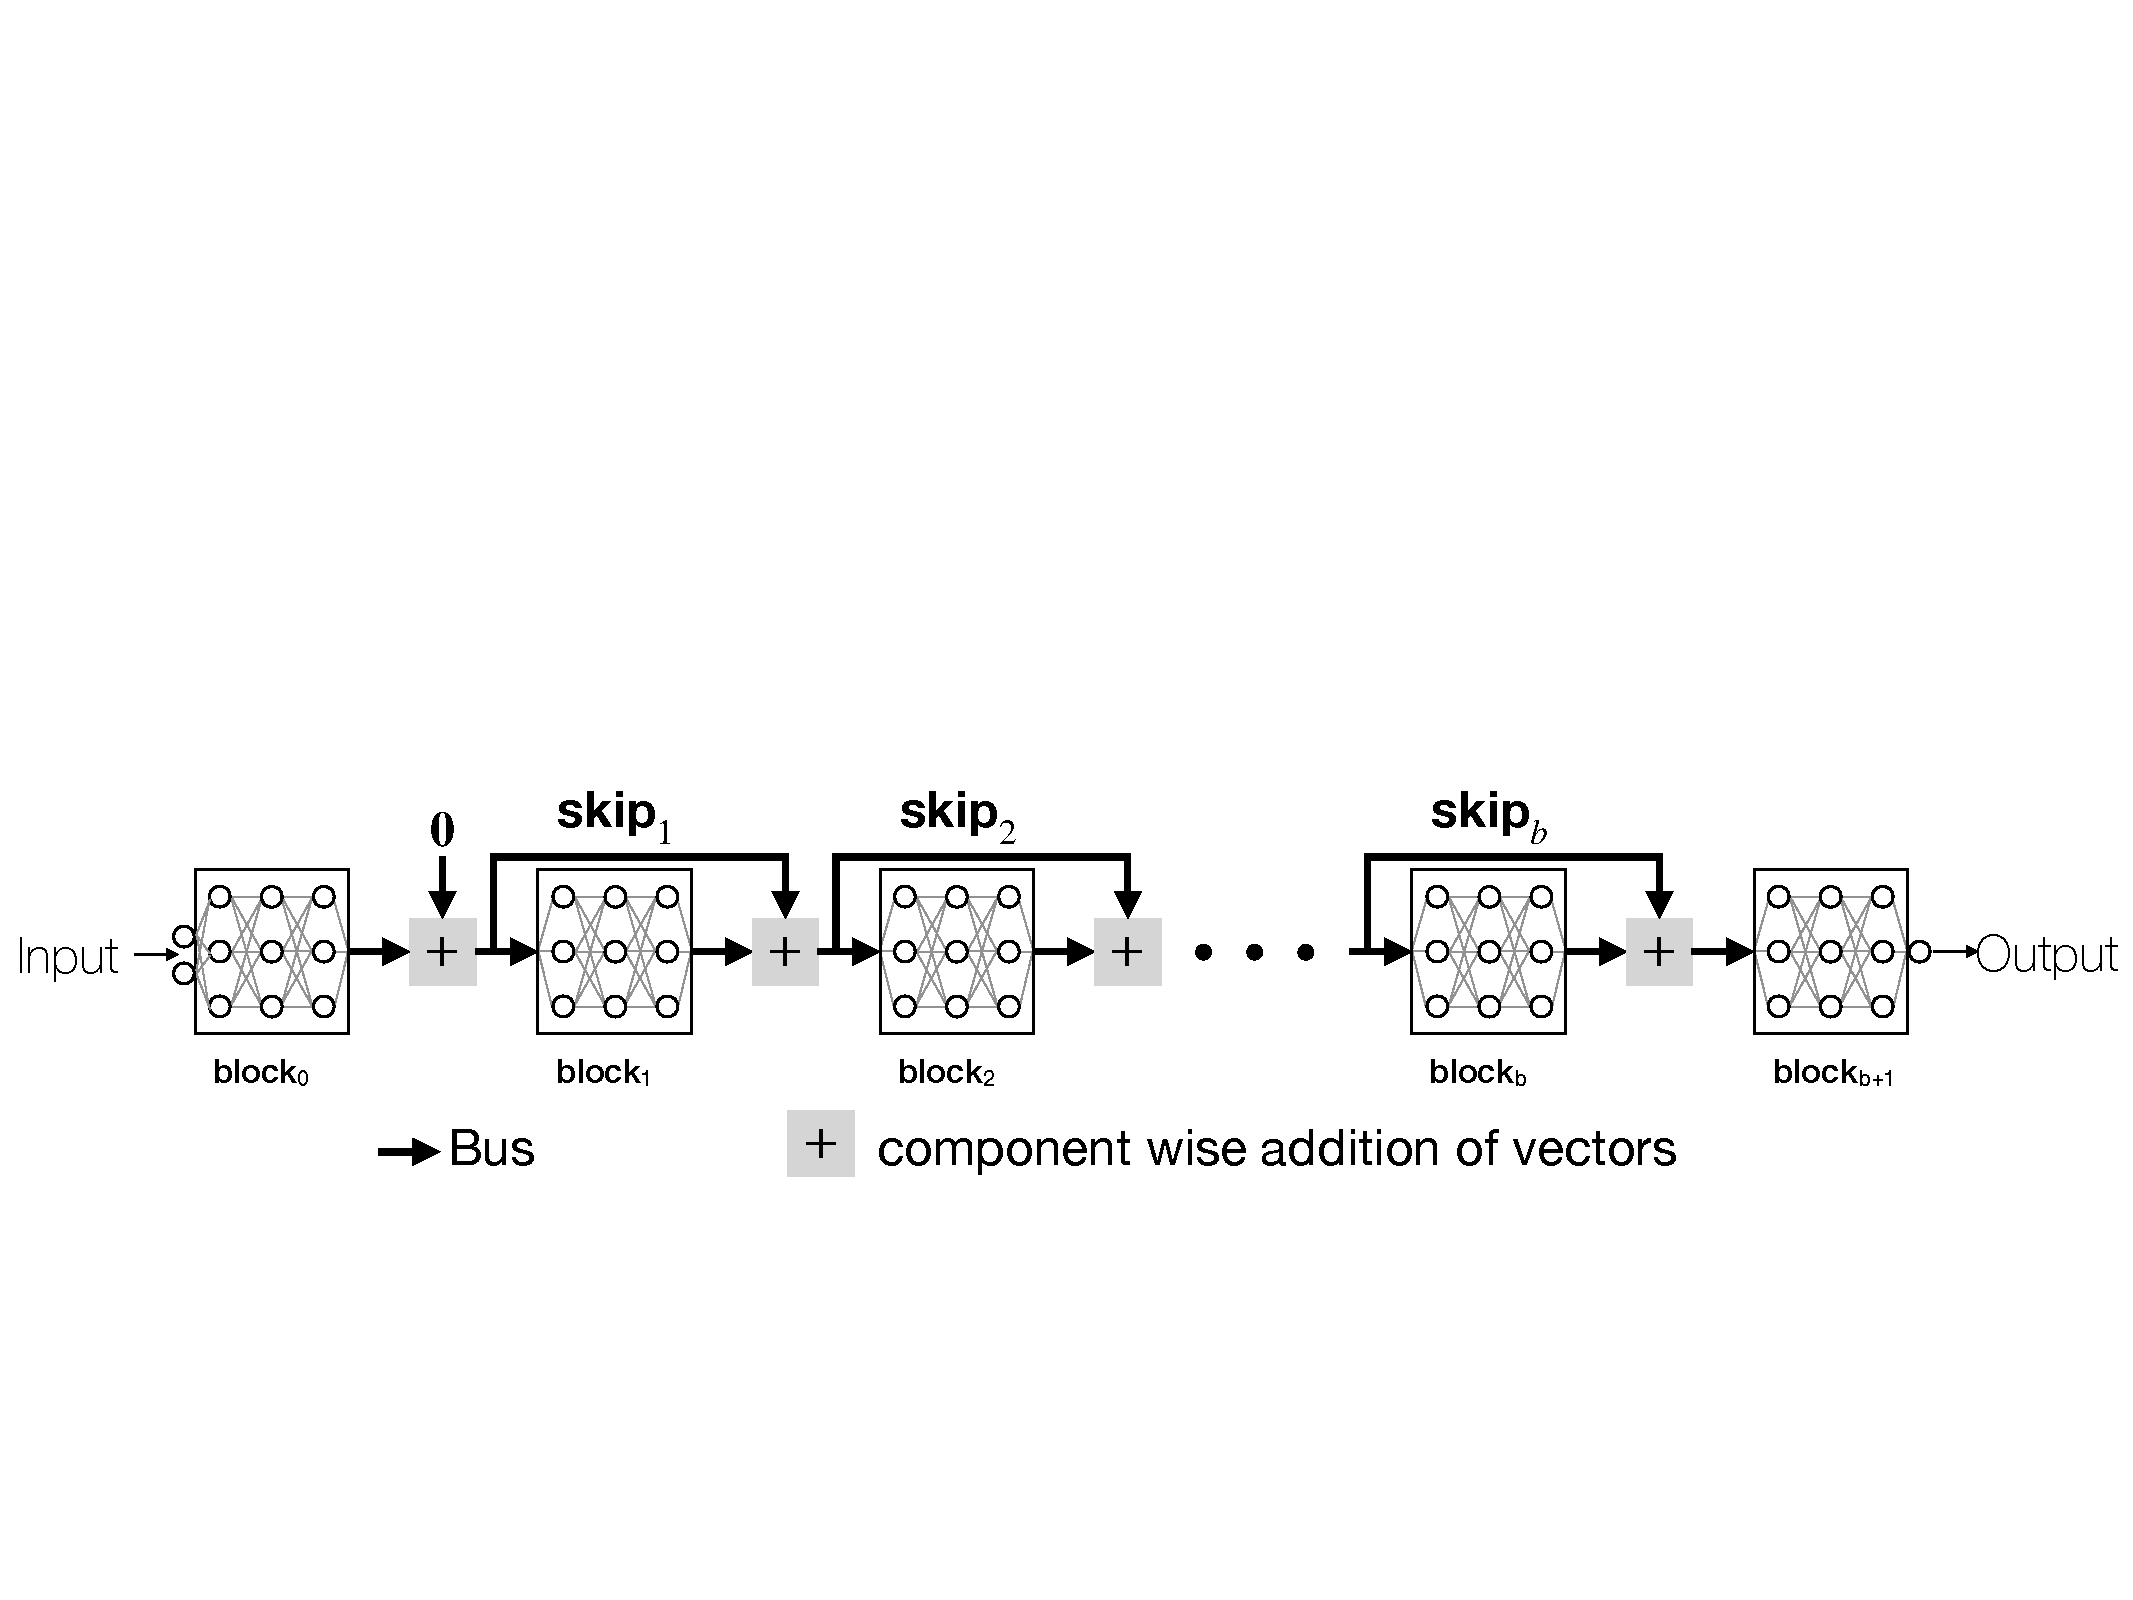
\includegraphics[scale=0.5]{figs/resnet.pdf}
}
\end{minipage}
\begin{minipage}{0.5\columnwidth}
\resizebox{\columnwidth}{!}{
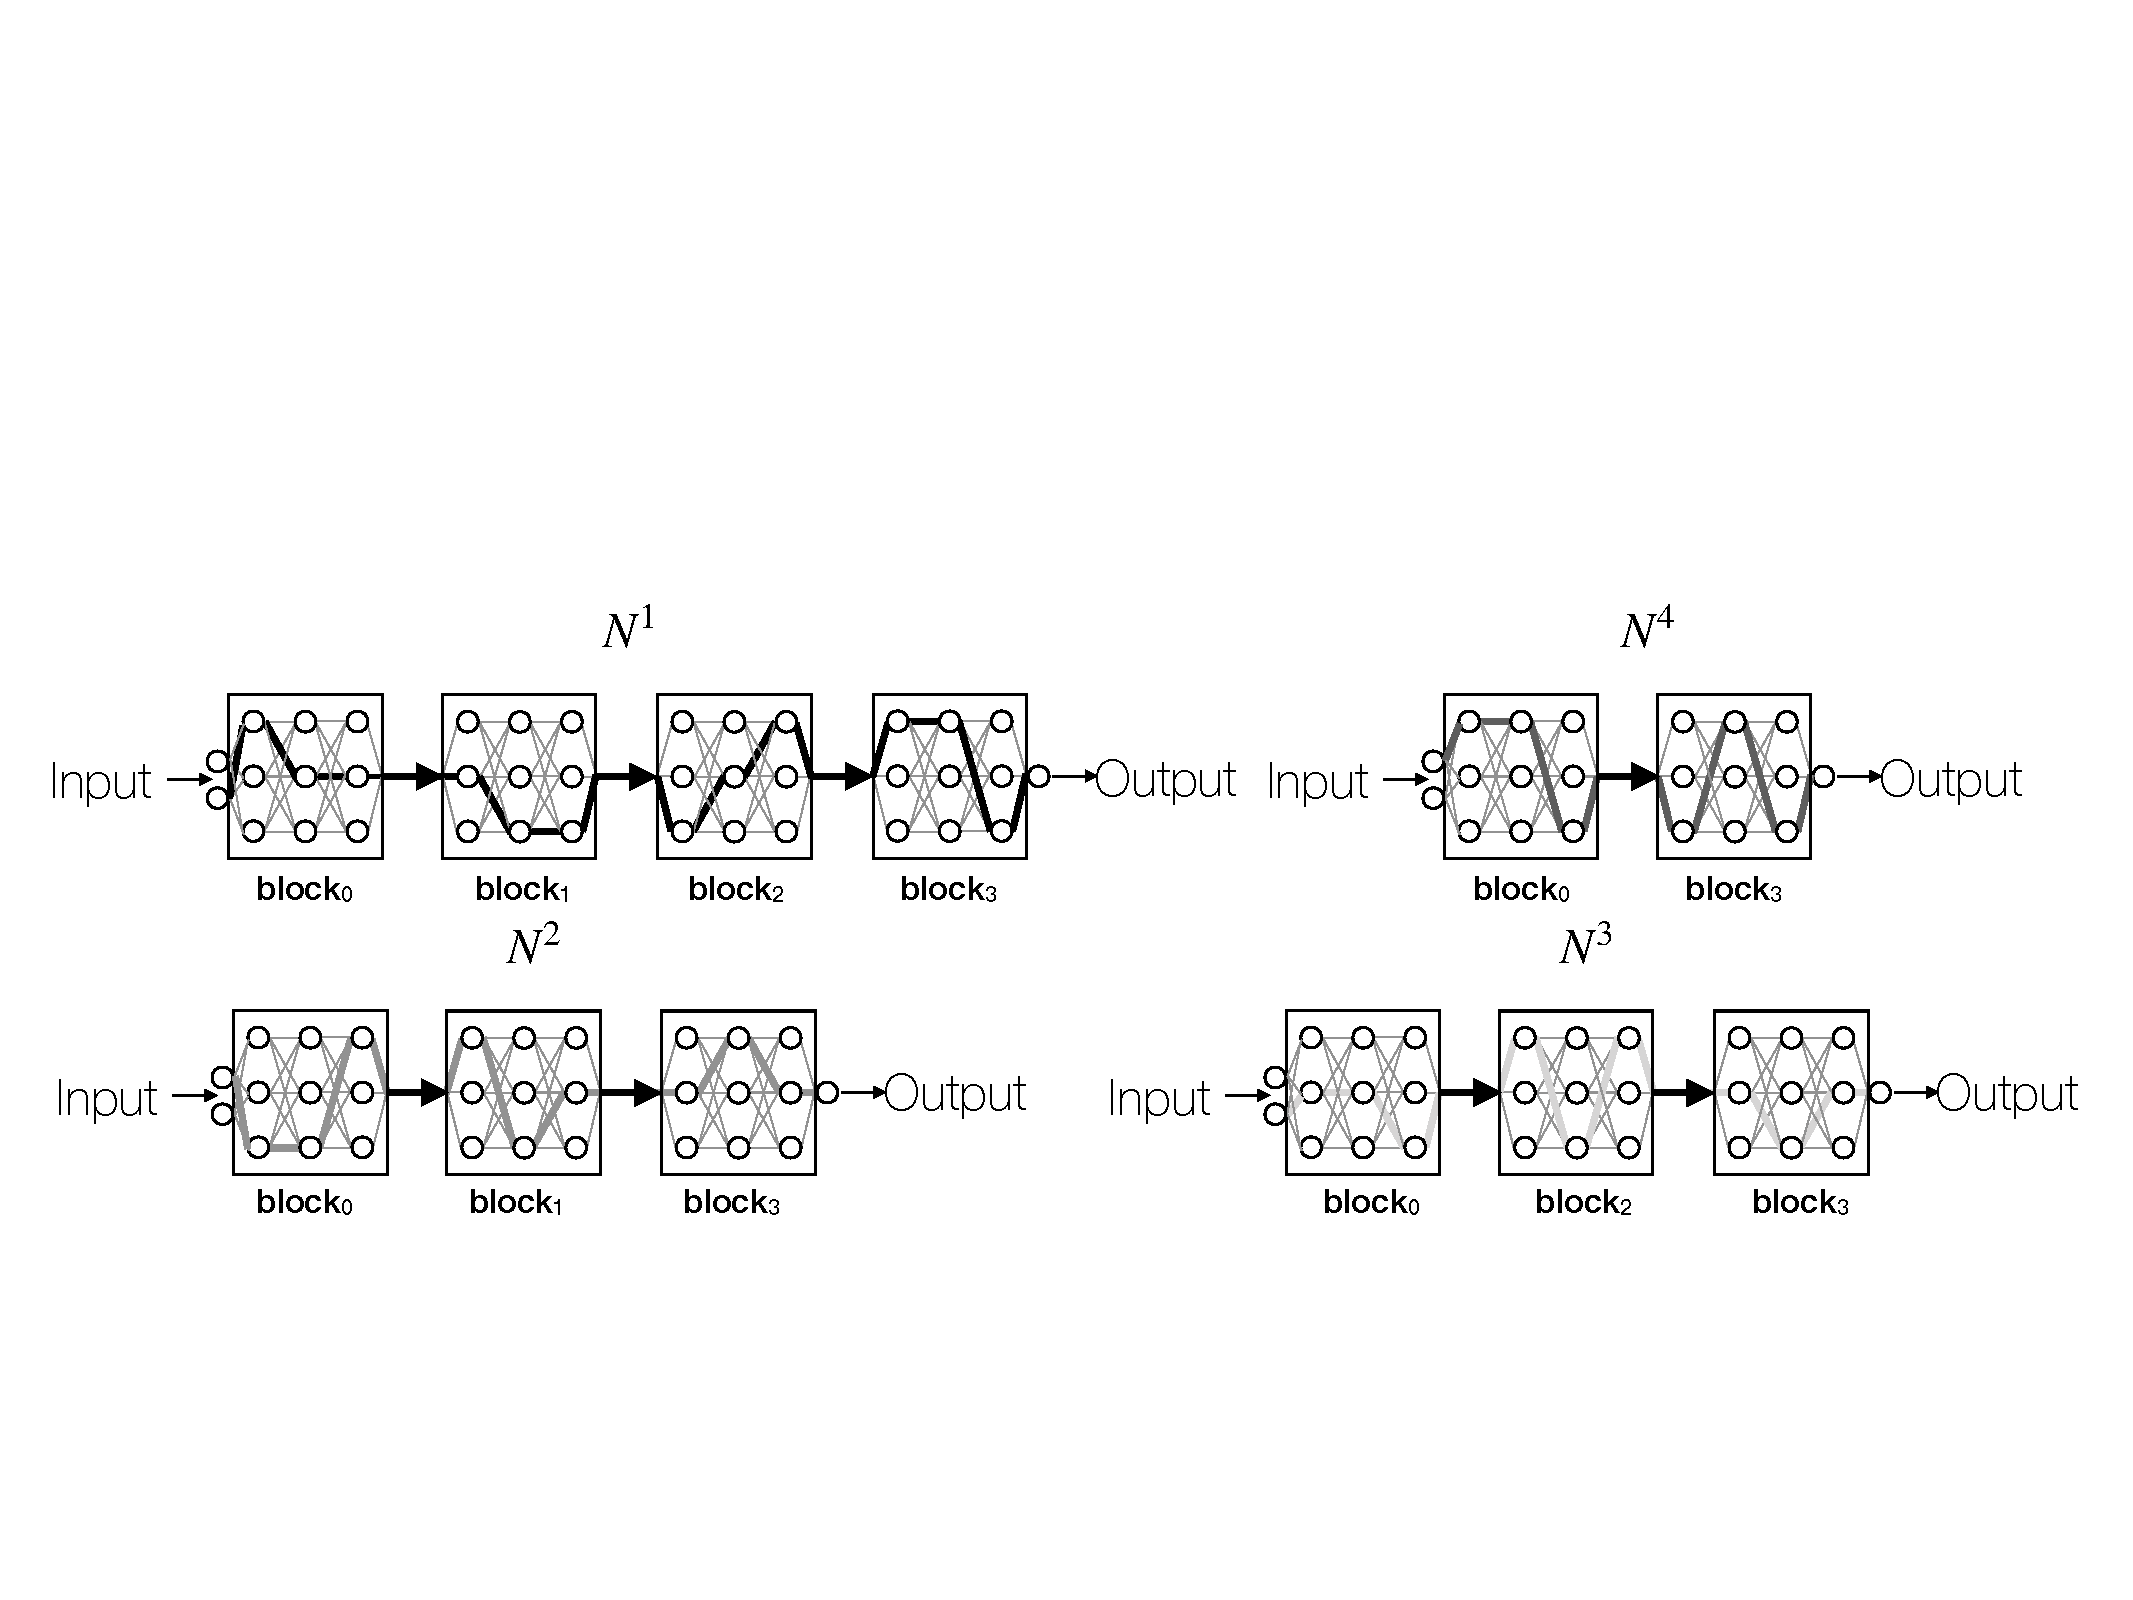
\includegraphics[scale=0.5]{figs/blocks.pdf}
}
\end{minipage}
\caption{\small{On the left is the ResNet with $b$ skip connections and $(b+2)$ blocks. On the right are the sub-FC networks $N^1$ obtained by skipping no blocks, $N^2$ and $N^4$ obtained by skipping block $1$ and $2$ respectively, and $N^3$ obtained by skipping both blocks $1$ and $2$.}}
\label{fig:resnet}
\end{figure}

\begin{definition}\label{def:subfcdnn}[Sub FC-DNNs]
Let $2^{[b]}$ denote the power set of $[b]$ and let $\J\in 2^{[b]}$ denote any subset of $[b]$. Define the`$\J^{th}$' sub-FC-DNN of the ResNet to be the fully connected network obtained by (i) including  $\text{block}_{j},\forall j\in \J$  and (ii) ignoring $\text{block}_{j},\forall j\notin \J$ (see \Cref{fig:resnet}).
\end{definition}
\begin{theorem}[Sum of Product of Kernels Theorem]\label{th:mainres} Let $H^{\J}_{\Tf_0}$ be the NPK of the $\J^{th}$ sub-FC-DNN, and $\bfc^{\J}$ be the associated constant. Under \Cref{assmp:main}, we have:
\begin{align*}
\kv_{\Tdgn_0}\ra \sum_{\J\in 2^{[b]}}  \bfc^{\J} H^{\J}_{\Tf_0}, \,\, \text{as}\,\,  w\ra\infty
\end{align*}
\end{theorem}
\textbf{Note.} The sub-FC-DNNs we refer to in \Cref{th:mainres} belong to (or are parts of) the feature network from which the gates are obtained. 
%\end{comment}